\documentclass[twoside]{book}

% Packages required by doxygen
\usepackage{fixltx2e}
\usepackage{calc}
\usepackage{doxygen}
\usepackage[export]{adjustbox} % also loads graphicx
\usepackage{graphicx}
\usepackage[utf8]{inputenc}
\usepackage{makeidx}
\usepackage{multicol}
\usepackage{multirow}
\PassOptionsToPackage{warn}{textcomp}
\usepackage{textcomp}
\usepackage[nointegrals]{wasysym}
\usepackage[table]{xcolor}

% NLS support packages
\usepackage[french]{babel}

% Font selection
\usepackage[T1]{fontenc}
\usepackage[scaled=.90]{helvet}
\usepackage{courier}
\usepackage{amssymb}
\usepackage{sectsty}
\renewcommand{\familydefault}{\sfdefault}
\allsectionsfont{%
  \fontseries{bc}\selectfont%
  \color{darkgray}%
}
\renewcommand{\DoxyLabelFont}{%
  \fontseries{bc}\selectfont%
  \color{darkgray}%
}
\newcommand{\+}{\discretionary{\mbox{\scriptsize$\hookleftarrow$}}{}{}}

% Page & text layout
\usepackage{geometry}
\geometry{%
  a4paper,%
  top=2.5cm,%
  bottom=2.5cm,%
  left=2.5cm,%
  right=2.5cm%
}
\tolerance=750
\hfuzz=15pt
\hbadness=750
\setlength{\emergencystretch}{15pt}
\setlength{\parindent}{0cm}
\setlength{\parskip}{0.2cm}
\makeatletter
\renewcommand{\paragraph}{%
  \@startsection{paragraph}{4}{0ex}{-1.0ex}{1.0ex}{%
    \normalfont\normalsize\bfseries\SS@parafont%
  }%
}
\renewcommand{\subparagraph}{%
  \@startsection{subparagraph}{5}{0ex}{-1.0ex}{1.0ex}{%
    \normalfont\normalsize\bfseries\SS@subparafont%
  }%
}
\makeatother

% Headers & footers
\usepackage{fancyhdr}
\pagestyle{fancyplain}
\fancyhead[LE]{\fancyplain{}{\bfseries\thepage}}
\fancyhead[CE]{\fancyplain{}{}}
\fancyhead[RE]{\fancyplain{}{\bfseries\leftmark}}
\fancyhead[LO]{\fancyplain{}{\bfseries\rightmark}}
\fancyhead[CO]{\fancyplain{}{}}
\fancyhead[RO]{\fancyplain{}{\bfseries\thepage}}
\fancyfoot[LE]{\fancyplain{}{}}
\fancyfoot[CE]{\fancyplain{}{}}
\fancyfoot[RE]{\fancyplain{}{\bfseries\scriptsize Généré le Lundi 29 Juin 2015 22\+:26\+:01 pour Ultimate Penguin Rampage par Doxygen }}
\fancyfoot[LO]{\fancyplain{}{\bfseries\scriptsize Généré le Lundi 29 Juin 2015 22\+:26\+:01 pour Ultimate Penguin Rampage par Doxygen }}
\fancyfoot[CO]{\fancyplain{}{}}
\fancyfoot[RO]{\fancyplain{}{}}
\renewcommand{\footrulewidth}{0.4pt}
\renewcommand{\chaptermark}[1]{%
  \markboth{#1}{}%
}
\renewcommand{\sectionmark}[1]{%
  \markright{\thesection\ #1}%
}

% Indices & bibliography
\usepackage{natbib}
\usepackage[titles]{tocloft}
\setcounter{tocdepth}{3}
\setcounter{secnumdepth}{5}
\makeindex

% Hyperlinks (required, but should be loaded last)
\usepackage{ifpdf}
\ifpdf
  \usepackage[pdftex,pagebackref=true]{hyperref}
\else
  \usepackage[ps2pdf,pagebackref=true]{hyperref}
\fi
\hypersetup{%
  colorlinks=true,%
  linkcolor=blue,%
  citecolor=blue,%
  unicode%
}

% Custom commands
\newcommand{\clearemptydoublepage}{%
  \newpage{\pagestyle{empty}\cleardoublepage}%
}


%===== C O N T E N T S =====

\begin{document}

% Titlepage & ToC
\hypersetup{pageanchor=false,
             bookmarks=true,
             bookmarksnumbered=true,
             pdfencoding=unicode
            }
\pagenumbering{roman}
\begin{titlepage}
\vspace*{7cm}
\begin{center}%
{\Large Ultimate Penguin Rampage \\[1ex]\large alpha\+\_\+0.\+1 }\\
\vspace*{1cm}
{\large Généré par Doxygen 1.8.10}\\
\vspace*{0.5cm}
{\small Lundi 29 Juin 2015 22:26:01}\\
\end{center}
\end{titlepage}
\clearemptydoublepage
\tableofcontents
\clearemptydoublepage
\pagenumbering{arabic}
\hypersetup{pageanchor=true}

%--- Begin generated contents ---
\chapter{Index des classes}
\section{Liste des classes}
Liste des classes, structures, unions et interfaces avec une brève description \+:\begin{DoxyCompactList}
\item\contentsline{section}{\hyperlink{class_u_p_r}{U\+P\+R} \\*La classe principale du programme }{\pageref{class_u_p_r}}{}
\item\contentsline{section}{\hyperlink{class_utils}{Utils} \\*Regroupe quelques fonctions d\textquotesingle{}utilité générale }{\pageref{class_utils}}{}
\end{DoxyCompactList}

\chapter{Index des fichiers}
\section{Liste des fichiers}
Liste de tous les fichiers avec une brève description \+:\begin{DoxyCompactList}
\item\contentsline{section}{include/\hyperlink{_u_p_r_8h}{U\+P\+R.\+h} }{\pageref{_u_p_r_8h}}{}
\item\contentsline{section}{include/\hyperlink{_utils_8h}{Utils.\+h} }{\pageref{_utils_8h}}{}
\item\contentsline{section}{src/\hyperlink{_u_p_r_8cpp}{U\+P\+R.\+cpp} }{\pageref{_u_p_r_8cpp}}{}
\item\contentsline{section}{src/\hyperlink{_utils_8cpp}{Utils.\+cpp} }{\pageref{_utils_8cpp}}{}
\end{DoxyCompactList}

\chapter{Documentation des classes}
\hypertarget{class_u_p_r}{}\section{Référence de la classe U\+P\+R}
\label{class_u_p_r}\index{U\+P\+R@{U\+P\+R}}


La classe principale du programme.  




{\ttfamily \#include $<$U\+P\+R.\+h$>$}

\subsection*{Attributs publics statiques}
\begin{DoxyCompactItemize}
\item 
static const int \hyperlink{class_u_p_r_a29b280f8a41e96854465f42ce303520b}{L\+A\+R\+G\+E\+U\+R\+\_\+\+E\+C\+R\+A\+N} = 800
\begin{DoxyCompactList}\small\item\em Largeur de l\textquotesingle{}écran (= 25 tiles). \end{DoxyCompactList}\item 
static const int \hyperlink{class_u_p_r_a68b3cf191ad71e0bea073c214f47b760}{H\+A\+U\+T\+E\+U\+R\+\_\+\+E\+C\+R\+A\+N} = 640
\begin{DoxyCompactList}\small\item\em Hauteur de l\textquotesingle{}écran (= 20 tiles). \end{DoxyCompactList}\item 
static S\+D\+L\+\_\+\+Window $\ast$ \hyperlink{class_u_p_r_a337a823f61ad23359193a2d031d3376e}{fenetre\+\_\+\+S\+D\+L} = N\+U\+L\+L
\begin{DoxyCompactList}\small\item\em La fenêtre du programme. \end{DoxyCompactList}\item 
static S\+D\+L\+\_\+\+Surface $\ast$ \hyperlink{class_u_p_r_af6f9d806062f3d722ac9e16ac6946814}{surface\+\_\+ecran} = N\+U\+L\+L
\begin{DoxyCompactList}\small\item\em La surface contenue par \hyperlink{class_u_p_r_a337a823f61ad23359193a2d031d3376e}{U\+P\+R\+::fenetre\+\_\+\+S\+D\+L}. \end{DoxyCompactList}\end{DoxyCompactItemize}


\subsection{Description détaillée}
La classe principale du programme. 

Contient la fenêtre ainsi que sa surface et son renderer. Contient également les diverses dimensions constantes utilisées dans le programme. 

\subsection{Documentation des données membres}
\hypertarget{class_u_p_r_a337a823f61ad23359193a2d031d3376e}{}\index{U\+P\+R@{U\+P\+R}!fenetre\+\_\+\+S\+D\+L@{fenetre\+\_\+\+S\+D\+L}}
\index{fenetre\+\_\+\+S\+D\+L@{fenetre\+\_\+\+S\+D\+L}!U\+P\+R@{U\+P\+R}}
\subsubsection[{fenetre\+\_\+\+S\+D\+L}]{\setlength{\rightskip}{0pt plus 5cm}S\+D\+L\+\_\+\+Window $\ast$ U\+P\+R\+::fenetre\+\_\+\+S\+D\+L = N\+U\+L\+L\hspace{0.3cm}{\ttfamily [static]}}\label{class_u_p_r_a337a823f61ad23359193a2d031d3376e}


La fenêtre du programme. 

Créée par \hyperlink{class_utils_a65fa5f629d47909dcd35b7194a394df5}{Utils\+::initialisation\+S\+D\+L()}.

Détruite par S\+D\+L\+\_\+\+Destroy\+Window() dans \hyperlink{class_utils_a1a1317e9deaac6dc1ad285d101b6f929}{Utils\+::quitter()}. \hypertarget{class_u_p_r_a68b3cf191ad71e0bea073c214f47b760}{}\index{U\+P\+R@{U\+P\+R}!H\+A\+U\+T\+E\+U\+R\+\_\+\+E\+C\+R\+A\+N@{H\+A\+U\+T\+E\+U\+R\+\_\+\+E\+C\+R\+A\+N}}
\index{H\+A\+U\+T\+E\+U\+R\+\_\+\+E\+C\+R\+A\+N@{H\+A\+U\+T\+E\+U\+R\+\_\+\+E\+C\+R\+A\+N}!U\+P\+R@{U\+P\+R}}
\subsubsection[{H\+A\+U\+T\+E\+U\+R\+\_\+\+E\+C\+R\+A\+N}]{\setlength{\rightskip}{0pt plus 5cm}const int U\+P\+R\+::\+H\+A\+U\+T\+E\+U\+R\+\_\+\+E\+C\+R\+A\+N = 640\hspace{0.3cm}{\ttfamily [static]}}\label{class_u_p_r_a68b3cf191ad71e0bea073c214f47b760}


Hauteur de l\textquotesingle{}écran (= 20 tiles). 

\hypertarget{class_u_p_r_a29b280f8a41e96854465f42ce303520b}{}\index{U\+P\+R@{U\+P\+R}!L\+A\+R\+G\+E\+U\+R\+\_\+\+E\+C\+R\+A\+N@{L\+A\+R\+G\+E\+U\+R\+\_\+\+E\+C\+R\+A\+N}}
\index{L\+A\+R\+G\+E\+U\+R\+\_\+\+E\+C\+R\+A\+N@{L\+A\+R\+G\+E\+U\+R\+\_\+\+E\+C\+R\+A\+N}!U\+P\+R@{U\+P\+R}}
\subsubsection[{L\+A\+R\+G\+E\+U\+R\+\_\+\+E\+C\+R\+A\+N}]{\setlength{\rightskip}{0pt plus 5cm}const int U\+P\+R\+::\+L\+A\+R\+G\+E\+U\+R\+\_\+\+E\+C\+R\+A\+N = 800\hspace{0.3cm}{\ttfamily [static]}}\label{class_u_p_r_a29b280f8a41e96854465f42ce303520b}


Largeur de l\textquotesingle{}écran (= 25 tiles). 

\hypertarget{class_u_p_r_af6f9d806062f3d722ac9e16ac6946814}{}\index{U\+P\+R@{U\+P\+R}!surface\+\_\+ecran@{surface\+\_\+ecran}}
\index{surface\+\_\+ecran@{surface\+\_\+ecran}!U\+P\+R@{U\+P\+R}}
\subsubsection[{surface\+\_\+ecran}]{\setlength{\rightskip}{0pt plus 5cm}S\+D\+L\+\_\+\+Surface $\ast$ U\+P\+R\+::surface\+\_\+ecran = N\+U\+L\+L\hspace{0.3cm}{\ttfamily [static]}}\label{class_u_p_r_af6f9d806062f3d722ac9e16ac6946814}


La surface contenue par \hyperlink{class_u_p_r_a337a823f61ad23359193a2d031d3376e}{U\+P\+R\+::fenetre\+\_\+\+S\+D\+L}. 

Permet d\textquotesingle{}y afficher du contenu en utilisant le double buffer.

Initialisée dans \hyperlink{class_utils_a65fa5f629d47909dcd35b7194a394df5}{Utils\+::initialisation\+S\+D\+L()}.

Elle n\textquotesingle{}a pas d\textquotesingle{}instructions de suppression explicites, elle est détruite par la fonction S\+D\+L\+\_\+\+Destroy\+Window() utilisée dans la fonction \hyperlink{class_utils_a1a1317e9deaac6dc1ad285d101b6f929}{Utils\+::quitter()}. 

La documentation de cette classe a été générée à partir des fichiers suivants \+:\begin{DoxyCompactItemize}
\item 
include/\hyperlink{_u_p_r_8h}{U\+P\+R.\+h}\item 
src/\hyperlink{_u_p_r_8cpp}{U\+P\+R.\+cpp}\end{DoxyCompactItemize}

\hypertarget{class_utils}{}\section{Référence de la classe Utils}
\label{class_utils}\index{Utils@{Utils}}


Regroupe quelques fonctions d\textquotesingle{}utilité générale.  




{\ttfamily \#include $<$Utils.\+h$>$}

\subsection*{Fonctions membres publiques statiques}
\begin{DoxyCompactItemize}
\item 
static bool \hyperlink{class_utils_a65fa5f629d47909dcd35b7194a394df5}{initialisation\+S\+D\+L} ()
\begin{DoxyCompactList}\small\item\em Initialise la S\+D\+L et ses principaux composants. \end{DoxyCompactList}\item 
static void \hyperlink{class_utils_a1a1317e9deaac6dc1ad285d101b6f929}{quitter} ()
\begin{DoxyCompactList}\small\item\em Détruit les composants restants de la S\+D\+L et quitte correctement les systèmes ouverts. \end{DoxyCompactList}\end{DoxyCompactItemize}


\subsection{Description détaillée}
Regroupe quelques fonctions d\textquotesingle{}utilité générale. 

\subsection{Documentation des fonctions membres}
\hypertarget{class_utils_a65fa5f629d47909dcd35b7194a394df5}{}\index{Utils@{Utils}!initialisation\+S\+D\+L@{initialisation\+S\+D\+L}}
\index{initialisation\+S\+D\+L@{initialisation\+S\+D\+L}!Utils@{Utils}}
\subsubsection[{initialisation\+S\+D\+L()}]{\setlength{\rightskip}{0pt plus 5cm}bool Utils\+::initialisation\+S\+D\+L (
\begin{DoxyParamCaption}
{}
\end{DoxyParamCaption}
)\hspace{0.3cm}{\ttfamily [static]}}\label{class_utils_a65fa5f629d47909dcd35b7194a394df5}


Initialise la S\+D\+L et ses principaux composants. 

\begin{DoxyReturn}{Renvoie}
T\+R\+U\+E si l\textquotesingle{}initialisation s\textquotesingle{}est correctement déroulée. 

F\+A\+L\+S\+E si il y a eu un problème avec l\textquotesingle{}initialisation de la S\+D\+L. 
\end{DoxyReturn}
\hypertarget{class_utils_a1a1317e9deaac6dc1ad285d101b6f929}{}\index{Utils@{Utils}!quitter@{quitter}}
\index{quitter@{quitter}!Utils@{Utils}}
\subsubsection[{quitter()}]{\setlength{\rightskip}{0pt plus 5cm}void Utils\+::quitter (
\begin{DoxyParamCaption}
{}
\end{DoxyParamCaption}
)\hspace{0.3cm}{\ttfamily [static]}}\label{class_utils_a1a1317e9deaac6dc1ad285d101b6f929}


Détruit les composants restants de la S\+D\+L et quitte correctement les systèmes ouverts. 



La documentation de cette classe a été générée à partir des fichiers suivants \+:\begin{DoxyCompactItemize}
\item 
include/\hyperlink{_utils_8h}{Utils.\+h}\item 
src/\hyperlink{_utils_8cpp}{Utils.\+cpp}\end{DoxyCompactItemize}

\chapter{Documentation des fichiers}
\hypertarget{_u_p_r_8h}{}\section{Référence du fichier include/\+U\+P\+R.h}
\label{_u_p_r_8h}\index{include/\+U\+P\+R.\+h@{include/\+U\+P\+R.\+h}}
{\ttfamily \#include $<$S\+D\+L.\+h$>$}\\*
{\ttfamily \#include $<$string.\+h$>$}\\*
Graphe des dépendances par inclusion de U\+P\+R.\+h\+:\nopagebreak
\begin{figure}[H]
\begin{center}
\leavevmode
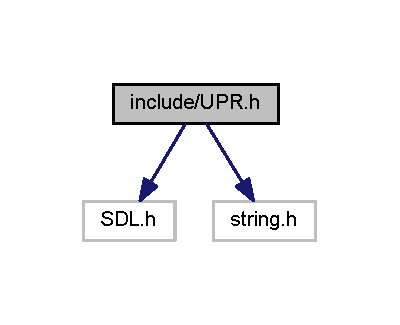
\includegraphics[width=192pt]{_u_p_r_8h__incl}
\end{center}
\end{figure}
Ce graphe montre quels fichiers incluent directement ou indirectement ce fichier \+:\nopagebreak
\begin{figure}[H]
\begin{center}
\leavevmode
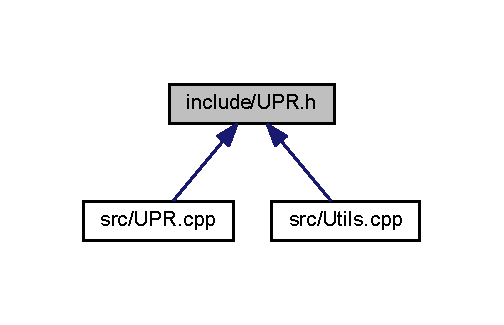
\includegraphics[width=242pt]{_u_p_r_8h__dep__incl}
\end{center}
\end{figure}
\subsection*{Classes}
\begin{DoxyCompactItemize}
\item 
class \hyperlink{class_u_p_r}{U\+P\+R}
\begin{DoxyCompactList}\small\item\em La classe principale du programme. \end{DoxyCompactList}\end{DoxyCompactItemize}

\hypertarget{_utils_8h}{}\section{Référence du fichier include/\+Utils.h}
\label{_utils_8h}\index{include/\+Utils.\+h@{include/\+Utils.\+h}}
Ce graphe montre quels fichiers incluent directement ou indirectement ce fichier \+:\nopagebreak
\begin{figure}[H]
\begin{center}
\leavevmode
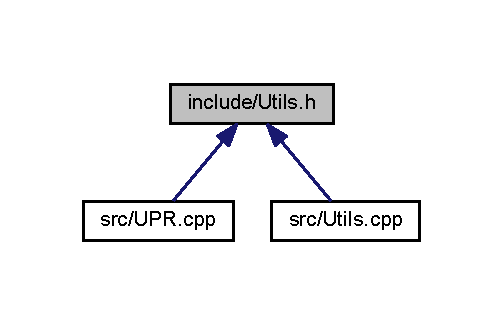
\includegraphics[width=242pt]{_utils_8h__dep__incl}
\end{center}
\end{figure}
\subsection*{Classes}
\begin{DoxyCompactItemize}
\item 
class \hyperlink{class_utils}{Utils}
\begin{DoxyCompactList}\small\item\em Regroupe quelques fonctions d\textquotesingle{}utilité générale. \end{DoxyCompactList}\end{DoxyCompactItemize}

\hypertarget{_u_p_r_8cpp}{}\section{Référence du fichier src/\+U\+P\+R.cpp}
\label{_u_p_r_8cpp}\index{src/\+U\+P\+R.\+cpp@{src/\+U\+P\+R.\+cpp}}
{\ttfamily \#include $<$iostream$>$}\\*
{\ttfamily \#include \char`\"{}U\+P\+R.\+h\char`\"{}}\\*
{\ttfamily \#include \char`\"{}Utils.\+h\char`\"{}}\\*
Graphe des dépendances par inclusion de U\+P\+R.\+cpp\+:\nopagebreak
\begin{figure}[H]
\begin{center}
\leavevmode
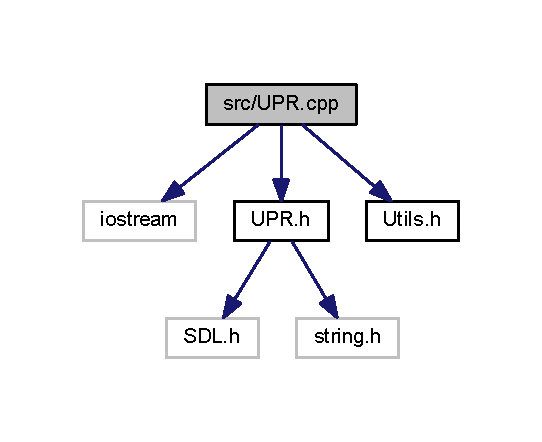
\includegraphics[width=260pt]{_u_p_r_8cpp__incl}
\end{center}
\end{figure}
\subsection*{Fonctions}
\begin{DoxyCompactItemize}
\item 
int \hyperlink{_u_p_r_8cpp_a700a0caa5b70a06d1064e576f9f3cf65}{main} (int argc, char $\ast$args\mbox{[}$\,$\mbox{]})
\begin{DoxyCompactList}\small\item\em La fonction main. \end{DoxyCompactList}\end{DoxyCompactItemize}


\subsection{Documentation des fonctions}
\hypertarget{_u_p_r_8cpp_a700a0caa5b70a06d1064e576f9f3cf65}{}\index{U\+P\+R.\+cpp@{U\+P\+R.\+cpp}!main@{main}}
\index{main@{main}!U\+P\+R.\+cpp@{U\+P\+R.\+cpp}}
\subsubsection[{main(int argc, char $\ast$args[])}]{\setlength{\rightskip}{0pt plus 5cm}int main (
\begin{DoxyParamCaption}
\item[{int}]{argc, }
\item[{char $\ast$}]{args\mbox{[}$\,$\mbox{]}}
\end{DoxyParamCaption}
)}\label{_u_p_r_8cpp_a700a0caa5b70a06d1064e576f9f3cf65}


La fonction main. 

Initialise la S\+D\+L grâces aux méthodes static de la classe \hyperlink{class_utils}{Utils}, lance la cinématique d\textquotesingle{}introduction puis le menu principal.

Une fois le jeu quitté, quitte la S\+D\+L correctement grâce à \hyperlink{class_utils_a1a1317e9deaac6dc1ad285d101b6f929}{Utils\+::quitter()}. 
\hypertarget{_utils_8cpp}{}\section{Référence du fichier src/\+Utils.cpp}
\label{_utils_8cpp}\index{src/\+Utils.\+cpp@{src/\+Utils.\+cpp}}
{\ttfamily \#include $<$iostream$>$}\\*
{\ttfamily \#include \char`\"{}U\+P\+R.\+h\char`\"{}}\\*
{\ttfamily \#include \char`\"{}Utils.\+h\char`\"{}}\\*
Graphe des dépendances par inclusion de Utils.\+cpp\+:
\nopagebreak
\begin{figure}[H]
\begin{center}
\leavevmode
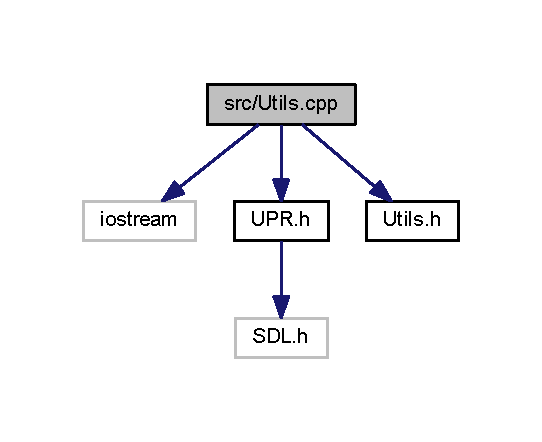
\includegraphics[width=260pt]{_utils_8cpp__incl}
\end{center}
\end{figure}

%--- End generated contents ---

% Index
\backmatter
\newpage
\phantomsection
\clearemptydoublepage
\addcontentsline{toc}{chapter}{Index}
\printindex

\end{document}
